
% to choose your degree
% please un-comment just one of the following
\documentclass[bsc,frontabs,twoside,singlespacing,parskip,deptreport]{infthesis}     % for BSc, BEng etc.
% \documentclass[minf,frontabs,twoside,singlespacing,parskip,deptreport]{infthesis}  % for MInf

\usepackage[utf8]{inputenc}
\usepackage{epigraph}
\usepackage{graphicx} %Added by Songbo
\usepackage{multirow}

% Flexible Qoute

\usepackage{epigraph,varwidth}

\renewcommand{\epigraphsize}{\small}
\setlength{\epigraphwidth}{0.6\textwidth}
\renewcommand{\textflush}{flushright}
\renewcommand{\sourceflush}{flushright}
% A useful addition
\newcommand{\epitextfont}{\itshape}
\newcommand{\episourcefont}{\scshape}

\makeatletter
\newsavebox{\epi@textbox}
\newsavebox{\epi@sourcebox}
\newlength\epi@finalwidth
\renewcommand{\epigraph}[2]{%
  \vspace{\beforeepigraphskip}
  {\epigraphsize\begin{\epigraphflush}
   \epi@finalwidth=\z@
   \sbox\epi@textbox{%
     \varwidth{\epigraphwidth}
     \begin{\textflush}\epitextfont#1\end{\textflush}
     \endvarwidth
   }%
   \epi@finalwidth=\wd\epi@textbox
   \sbox\epi@sourcebox{%
     \varwidth{\epigraphwidth}
     \begin{\sourceflush}\episourcefont#2\end{\sourceflush}%
     \endvarwidth
   }%
   \ifdim\wd\epi@sourcebox>\epi@finalwidth 
     \epi@finalwidth=\wd\epi@sourcebox
   \fi
   \leavevmode\vbox{
     \hb@xt@\epi@finalwidth{\hfil\box\epi@textbox}
     \vskip1.75ex
     \hrule height \epigraphrule
     \vskip.75ex
     \hb@xt@\epi@finalwidth{\hfil\box\epi@sourcebox}
   }%
   \end{\epigraphflush}
   \vspace{\afterepigraphskip}}}
\makeatother

% End Flexiable Qoute


\begin{document}

\title{Building Coherent Open-domain Dialogue Systems Using Neural Networks}

\author{Songbo Hu}

% to choose your course
% please un-comment just one of the following
\course{Artificial Intelligence and Computer Science}
%\course{Artificial Intelligence and Software Engineering}
%\course{Artificial Intelligence and Mathematics}
%\course{Artificial Intelligence and Psychology }   
%\course{Artificial Intelligence with Psychology }   
%\course{Linguistics and Artificial Intelligence}    
%\course{Computer Science}
%\course{Software Engineering}
%\course{Computer Science and Electronics}    
%\course{Electronics and Software Engineering}    
%\course{Computer Science and Management Science}    
%\course{Computer Science and Mathematics}
%\course{Computer Science and Physics}  
%\course{Computer Science and Statistics}    

% to choose your report type
% please un-comment just one of the following
%\project{Undergraduate Dissertation} % CS&E, E&SE, AI&L
%\project{Undergraduate Thesis} % AI%Psy
\project{4th Year Project Report}

\date{\today}

\abstract{
Add abstract later.
}

\maketitle

\section*{Acknowledgements}
Acknowledgements go here. 

\tableofcontents

%\pagenumbering{arabic}

\chapter{Introduction}

\epigraph{When was Alan Turing born? \\
Alan Turing was born on Sunday 13 June 1912. \\
Where was he born? \\
Alan Turing was born in Warrington Lodge. \\
Who is his father? \\
Julius Mathison Turing is Alan Turing's father.\\
When was he born? \\
Julius Mathison Turing was born 9 November 1873. \\
Where? \\
You're at Edinburgh, Scotland.
}{\textit{Songbo and Siri 2020}}

A dialogue system is a conversational agent that can converse with humans in natural language. It can help us solve many tedious tasks effectively or bring entertainment value to our daily life. Recent advances in dialogue systems (such as virtual assistants\cite{alexa,cortana,siri}) enable us to engage in natural conversational interactions with computers. It substantially increases the accessibility of state of the art technologies to people with diverse backgrounds. And for those with impairments, it could transform their daily living into a journey toward capability instead of disability.

Since Alan Turing published his landmark work in 1950\cite{turing1950computing}, the intelligence level of a machine is described as how well the machine is able to fool a human into believing that it, the machine, is a human based on its text responses. If a human is unable to distinguish the difference between the machine from a human, the machine is said to have passed the Turing test. We could say such a machine signifies a significantly high level of intelligence of an AI. It has been the goal for the development of dialogue systems for decades and various attempts have been proposed to pass the Turing test. Recently, advances in neural network based language models enable us to learn entire dialogue models directly from conversational data. Although we improve the performance of neural models by increasing the number of parameters and training with more data, we are still far from our goal. Most of the previous systems have failed to model the longer prior context of the conversation adequately, thereby creating a situation where extended dialogues rapidly become incoherent and unnatural sounding, with repetition being a key problem. 

As I demonstrated in the example conversation at the beginning, humans tend to utilise linguistic patterns, such as anaphora and sluicing to reduce repetitions. In contract, dialogue systems rarely produces pronouns and unable to model elided construction therefore produce unnatural speech in the context. For example, in order to answer the second question ("Where was he born?"), humans are able to interpret the anaphora (He refers to Alan Turing.) and produce a short answer (In Warrington Lodge.), in contrast to Siri's heavy and verbose response. The challenge for the Apple's inhouse system here is to know when such an answer conveys the intended content, and when it doesn't. The system has to make a decent decision on when content can be elided while still ensuring that the user can easily interpret the system's message and retrieve that message accurately. In addition, a wrong interpretation of a question could lead to an unhelpful and diverged response. Siri fails to use context to parse fragments and understand the sluicing in the final question. The misunderstanding of the context leads to a complete unhelpful and unrelated response. The lack of reliable systematic analysis of such linguistic patterns and the inadequate representation of the context are the main reasons for the unnaturalness. It is a problem which need to be adequately solved before our agents could look forward to attempting the Turing test.

In this section, we will briefly review the recent development of dialogue systems. Specifically, we will discuss two types of dialogue systems: the chit-chat dialogue system (known as chat bots), and the task-oriented dialogue system.  We will focus in this thesis on machine learning approaches to developing such systems, rather than the use of hand-crafted rules, since the former methods are now dominant and the latter are highly brittle and restricted to toy domains. We will discuss their architectures, pros and cons, and their main limitations to achieve coherent open-domain conversations. The majority of this thesis is about how to create an environment for neural models to learn linguistic patterns within coherent extended dialogues and how to integrate these models into the existing dialogue systems. It constitutes a first step towards modelling coherent open-domain conversations and will potentially enable the existing dialogue systems utilising valuable linguistic information to produce coherent responses.

\section {A Brief Review of Existing Dialogue Systems}

\subsection{The Chit-chat Dialogue System}

The chit-chat dialogue systems are usually called chatbots. These systems are designed and implemented to carry extended conversations with the goal of mimicking the ‘chats’ characteristic of informal human-human interaction\cite{jurafsky2019speech}. They are mainly aiming to provide entertainment value. Existing chatbots majorly fall into the following subcategories: the rule-based systems, the corpus-based systems, as will be discussed in order below.

\subsubsection*{The Rule-based Systems}

Instead of letting machines to learn the conversation strategy from human behaviours, we could ask humans to encode these human intelligence directly as rules and ask machines to interpret them. Dialogue agents could use these rules to generate dialogue utterances effectively. Normally, a message input will be processed by a set of carefully pre-defined rules e.g., a key-word look-up dictionary, if-else conditions, or more sophisticated machine learning classifiers\cite{jiweilithesis}. Consequently, the dialogue agent would produce a natural language response by outputting an utterance in storage, manipulating the input message or selecting some related historical contexts based on these rules.

\begin{figure}[h]
    \centering
    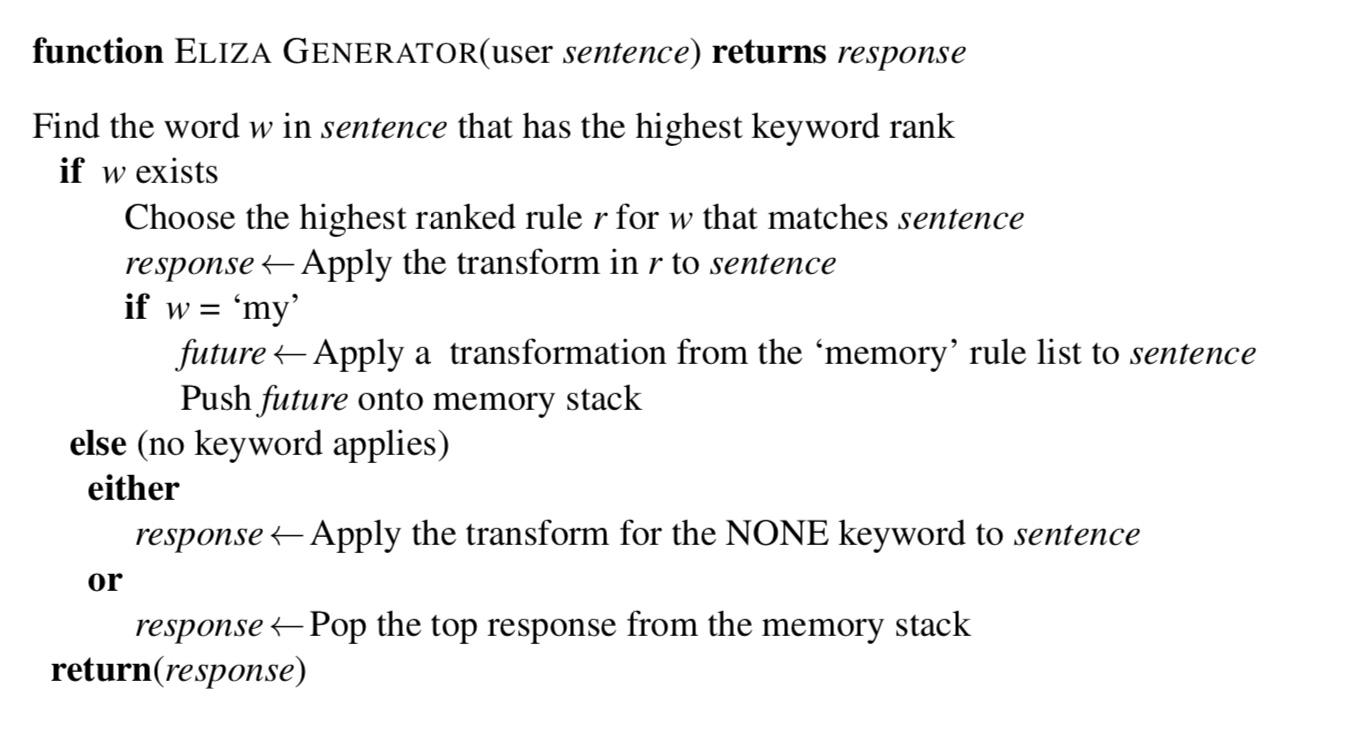
\includegraphics[width=0.9\textwidth]{elizarule.jpeg}
    \caption{A simplified sketch of the ELIZA algorithm.}
    \label{fig:elizarule}
\end{figure}

There are many well-known rule-based dialogue systems in history, such as ELIZA\cite{weizenbaum1966eliza}, ALICE\cite{wallace1995artificial}. There are also languages such as Artificial Intelligence Markup Language(AIML), which provides an effect tool to write sophisticated conversations logic in a machine-readable format\cite{wallace1995artificial}.

The development of rule-based systems is a important milestone in developing modern dialogue systems. They demonstrate how easy to fool a user into thinking there is intelligence in the machines behaviour when in fact there is no understanding and comprehension at all. Consequently, their drawbacks are obvious: rule-based systems predominantly rely on the set of pre-defined rules and these rules have to be carefully designed and implemented. Building a sophisticated rule-based system is very expensive because the number of these rules escalates rapidly. Rule-based systems do not have the ability to understand human languages, nor do they know how to generate meaningful natural language utterances\cite{jiweilithesis}. Consequently, they are very brittle and only able to conduct very superficial conversations. Despite the lack of intelligence, even with the recent rapid development of large fancy neural network architecture and increasing number of conversational corpora, these rule-based dialogue systems could always provide a very strong baseline.


\subsubsection*{The Corpus-based Systems}

Coding conversations logic manually is astronomically expensive and infeasible for many applications. Corpus-based dialogue system could potentially mitigate this issue by mining conversations of human-human conversations, or sometimes mining the human responses from human-machine conversations, instead of using hand-built rules. These data-driven approaches are becoming widely popular due to the increasing computing power and the creation of large scale conversational dataset. 

There are two common architectures for such system:  information retrieval (IR), and machine learned sequence transduction. Due to the limitation that IR-based chatbots can only mirror training data, it is often to treat response generation as a machine translation task which transduces from the user’s prior turn to the system’s turn. This method offers the promise of scalability and language-independence, together with the capacity to capture contextual dependencies in a way not possible with IR-based approaches.

\begin{figure}[h]
    \centering
    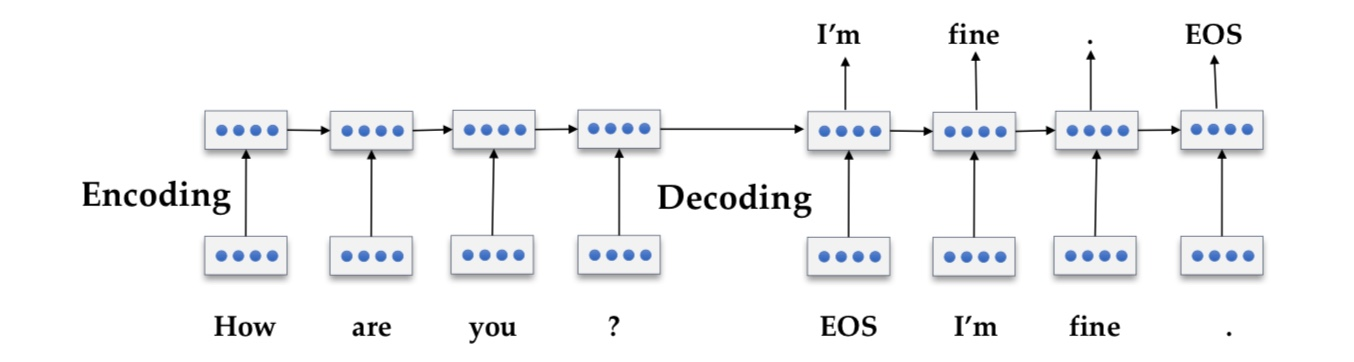
\includegraphics[width=0.9\textwidth]{seq2seq.jpeg}
    \caption{A sequence to sequence model for neural response generation.\cite{jurafsky2019speech}}
    \label{fig:seq2seq}
\end{figure}

This idea was firstly developed by Ritter et al\cite{ritter2011data}. (cited in Jurafsky and Martin\cite{jurafsky2019speech}) using phrase-based machine translation to translate a user turn to a system response. In 2015, transduction models for response generation were modelled instead using encoder-decoder (seq2seq) models\cite{shang2015neural,strub2017end,sordoni2015neural}. However, the simple seq2seq generation architecture is unable to model the prior context of the conversation. Serban et al\cite{serban2016building} suggests a hierarchical (HRED) model that summarizes information over multiple prior turns. This model consists of two recurrent neural networks (RNNs) stacked on top of each other: one is a sentence-level RNN which encodes each utterance into a fixed length vector, while a conversation-level RNN takes as input each utterance vector and outputs a vector that summarizes the conversation so far. The vector is mapped back to text using a recurrent decoder. This gives a way for the previous information to be passed to future turns as hidden states\cite{lowe2017training}.

\begin{figure}[h]
    \centering
    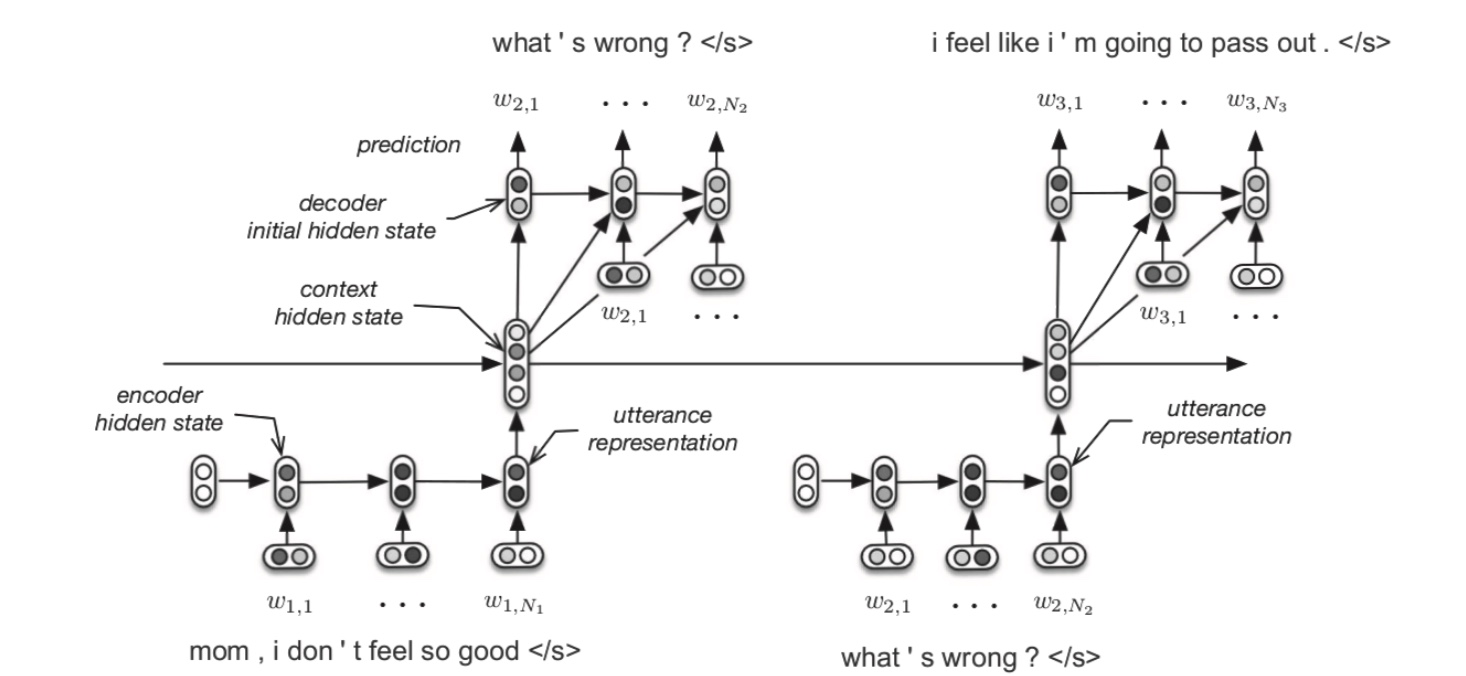
\includegraphics[width=0.9\textwidth]{HERD.jpeg}
    \caption{The computational graph of the HRED architecture for a dialogue composed of three turns.}
    \label{fig:HERD}
\end{figure}

However, even if one has access to an enormous dataset for training, there is still a significant proportion of unseen dialogue states. Techniques, such as smoothing, can only help to a limited extent, because of the radical extent to which data is sparse. Consequently, generating responses using end-to-end methods tends to generate generic, uninformative and non-coherent replies (e.g., generating ``I don’t know." regardless of the context). In addition, encoder-decoder response generators focus on generating single responses, instead of forming a coherent continuous conversation\cite{jurafsky2019speech}. Humans could easily notice these unnatural and mechanical responses (e.g. the Siri conversation above). Techniques, such as Reinforcement learning (RL) and adversarial networks, will be introduce in Chapter 2 to address this issue\cite{li2017adversarial,li2016deep}.

\subsection{The Goal-oriented Dialogue System}

 Goal-oriented dialogue systems are sometimes also called task-based dialogue systems, in which they converse with users to help complete tasks like making a restaurant reservation, booking a hotel or setting up an alarm. Famous examples of such agents are digital assistants (Siri, Alexa, Google Home, Cortana, et.) which can be viewed as a combination of chatbots and goal-oriented dialogue system. With the power of cloud computing and internet of things technologies, these conversations AIs are changing our daily life and developing a 10 billion pounds worth industry. Here, I would like to introduce the architectures of existing statistical spoken dialogue systems (hereafter SDSs) and their main challenges to perform coherent conversations in an open domain. 

\begin{figure}[h]
    \centering
    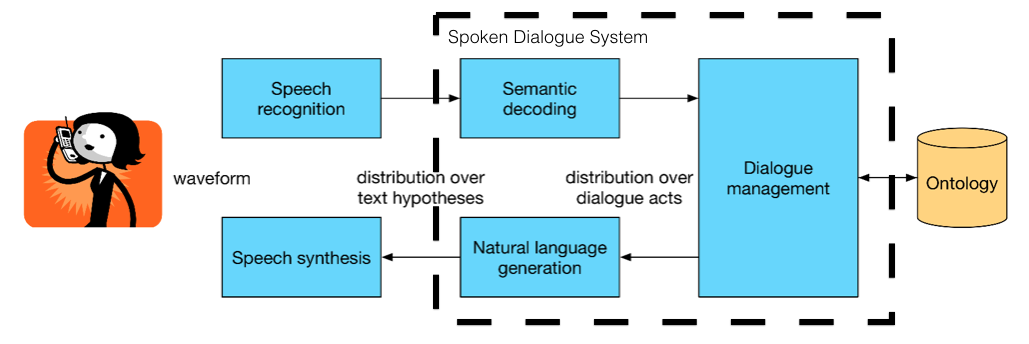
\includegraphics[width=0.80\textwidth]{sds.png}
    \caption{Architecture of a Spoken Dialogue System.\cite{gasic}}
    \label{fig:sds}
\end{figure}

Current SDSs have three key components which are shown as Figure\ref{fig:sds}. A semantics decoder decodes the meaning in utterances into dialogue acts which describe the current intention of the user, for example, confirm(food=Korean). Then, a dialogue manager, which usually consists of a belief tracker and a policy network, will keep track of the belief states and produce a dialogue act as the response. The dialogue manager treats dialogue generation as a partially observable Markov decision process (POMDP)\cite{williams2007partially,young2013pomdp,young2010hidden} which explicitly models the uncertainty natural of human conversations with Bayesian methods. Such framework provides robustness against the errors created by the speech recognition. Later a semantic encoder (natural language generator) will map this act back into a natural language response.

However, keeping track of the belief states under such a framework presents a tough challenge. Exact model representation is infeasible due to the limitation of computational complexity\cite{young2013pomdp}. Carefully constructed approximation and additional independent assumption are needed. For example, if we are willing to find an expensive 5-star hotel in the city center, in order to make the inference practical, we have to assume that there is no relation between a hotel is expensive and it is a 5-star hotel. It is clearly not true. In addition, as shown in Figure\ref{fig:sds}, pre-defined ontology is needed in order to keep track of the dialogue state. This makes the existing dialogue system infeasible to perform conversations in an open-domain. One research direction would be building a SDS which can support a natural conversation about any topic within a wide coverage Knowledge Graph (KG). This forms the definition of an open-domain spoken dialogue system\cite{opendomain}.




\section {Thesis Outline}

In this thesis, we mainly focus on creating a framework in which neural models could learn linguistic patterns within in extended coherent dialogues.

Firstly, we explore how to build such a framework by designing, collecting and annotating a conversational dataset. This dataset consists of extended coherent dialogues of questions and responses. These dialogues should describe the relations within a knowledge graph with clear links between the phrases in the questions to nodes in a knowledge graph. Secondly, we analyse the collected dataset statistically in order to investigate how human behave differently under different context in different domain. Later, we will introduce a proposed neural model to model these linguistic patterns and how the existing dialogue systems could benefit from such a model.

We start off by providing background knowledge on language modelling, training dialogue models, available dataset and how to evaluate such dialogue models in Chapter 2. In chapter 3,4, I will describe the design and creation of our framework in details and perform analysis to figure out the common patterns within these dialogues. Chapter 5,6 will introduce our proposed neural models and methods to integrate them into current dialogue systems. We will discuss our finding in Chapter 7 and mention some further improvement to our framework in Chapter 8.

\chapter{Background}

In this chapter, we describe the existing resources and methods to build a neural dialogue model. After that, we briefly introduce the existing approaches to deploy machine learning to do dialogue modelling and techniques we could use to improve the model performance. Finally, the later sections investigate the evaluation metrics of neural dialogue models.

\section{Corpora for Training Dialogue Models}

Humans perform dialogues with different purposes, under different situations and in different modalities. There is a vast amount of data available documenting human communications with different types of dialogue interactions. Some of these data are collected as corpora and these corpora are classified into different categories. Each category has different characteristics, utilities and applications. In order to make the most of the available resources, we discuss the important distinctions between each type of dialogue corpora: whether the corpus features constrained or unconstrained dialogues; whether a corpus is written, spoken; whether a corpus features human-human interactions or human-machine interactions. Afterwards, I give a brief summary about public available corpora for each type of dialogue corpora.


\subsection{Chit-chat or Goal-oriented}

People use different languages for different purposes. We may want to call an airliner to book a ticket chat with our friends to share our ideas. The purpose of our dialogues will have a significant influence on the language we use. Similarly, the way in which a dialogue corpus is collected can also have a significant influence on the model we built from. Some conversations are relatively causal, informal and unconstrained, which we usually call them chitchat. Most existing chit-chat datasets are aiming to mimic spontaneous and unplanned spoken interactions between humans. Consequently, they are also referred as Spontaneous (Unconstrained) Corpora. Typically, chit-chat corpora are close to the generally unplanned nature of most spoken interactions between humans. Another large proportion of existing corpora focus on a particular topic or intend to solve a specific task. In such situations, the task or topic is pre-specified and participants are discouraged from deviating from the topic. We refer to these as Task-Oriented or Constrained Dialogue Corpora.

Spontaneous Corpora bear a close resemblance to natural dialogues — that is, they are close to the generally unplanned nature of most spoken interactions between humans. 


In the latter case — that of constrained dialogues — some experimental conditions in which dialogues were collected can result in unnatural behaviours that do not correlate well to the true typical dialogue patterns of human-human interaction in day-to-day settings. 


\subsection{Chit-chat Dataset}


\subsubsection{Switchboard dataset}

The Switchboard dataset\cite{godfrey1992switchboard} is one of the most one of the most influential spoken corpora. This dataset consists of approximately 2,500 dialogues from phone calls, along with word- by-word transcriptions, with about 500 different speakers. A computer-driven robot operator system introduced a topic for discussion between two participants, and recorded the resulting conversation. This dataset consists of approximately 2,500 dialogues from phone calls, along with word-by-word transcriptions, with about 500 different speakers. A computer-driven robot operator system introduced a topic for discussion between two participants, and recorded the resulting conversation. About 70 casual topics were provided, of which about 50 were frequently used. The corpus was originally designed for training and testing various speech processing algorithms; however, it has also been used for a wide variety tasks.

\subsubsection{British National Corpus}

Another important dataset is the British National Corpus (BNC)\cite{leech1992100}), which contains approximately 10 million words of dialogue. These were collected in a variety of contexts ranging from formal business or government meetings, to radio shows and phone-ins. Although most of the conversations are spoken in nature, some of them are also written. BNC covers a large number of sources, and was designed to represent a wide cross-section of British English from the late twentieth century. The corpus also includes part-of-speech (POS) tagging for every word. The vast array of settings and topics covered by this corpus renders it very useful as a general-purpose spoken dialogue dataset.

\subsubsection{Twitter}

With the enormous increase of Internet users all over the world and the rapid development of social medias, a tremendous amount of conversations are recorded on the Internet. Several corpora of spontaneous micro-blogging conversations have been collected, such as the 
Twitter Corpus from Ritter et al.\cite{ritter2010unsupervised}, which contains 1.3 million post-reply pairs extracted from Twitter. The corpus was originally constructed to aid in the production of unsupervised approaches to modeling dialogue acts. Larger Twitter corpora have been collected. The Twitter Triples Corpus\cite{sordoni2015neural} is one such example, with a described original dataset of 127 million context-message-response triples.

\subsection{Task-Oriented}



\subsubsection{Air Travel Information System Pilot Corpus}

The ATIS (Air Travel Information System) Pilot Corpus\cite{hemphill1990atis} is one of the first human-machine corpora. It consists of interactions, lasting about 40 minutes each, between human participants and a travel-type booking system, secretly operated by humans. This dataset contains 1041 utterances.

\subsection{MulltiOZ}

MulltiOZ

\subsection{GuessWhat!}
GuessWhat!
FOILIT

\subsection{CoQA}
CoQA
Complex Sequential Question Answering\cite{saha2018complex}
The size of these datasets is a big advantage compared to other corpora, which makes them suitable to train neural methods and adapt unsupervised learning. However, such corpora are relatively noisy. The Twitter Corpus has an enormous amount of typos, slang, and abbreviations. Due to the 140-character limit in this dataset, tweets are often very short and compressed. In addition, such conversations also may depend on external unobserved events, because most of the twitters often implicitly refer to recent public events outside the conversation.

\section{Dialogue Model Evaluation}


\subsection{Intrinsic Evaluation}
Perplexity
BLEU Score
...
Talk about their limitation.


\subsection{Extrinsic Evaluation}

Evaluation on downstream tasks.


Question Answering Tasks. Use precision and rcall or F1 Score as its evaluation metrics.

\subsection{Human Evaluation}

Best but expensive.


\chapter{Extended Dialogues Grounded on Knowledge Graph: A Corpus}

In this chapter, I intend design and collect a novel corpus which creates a framework for neural models to learn various linguistics patterns. In contrast to previous studies\cite{reddy2019coqa,de2017guesswhat,saha2018complex,shekhar2017foil}, in which the conversations are grounded on images or short paragraphs, our dataset contains extended coherent dialogues of questions and responses that are information in a knowledge graph. I will introduce the design principle, my implementation, the data collection and annotation procedure of my framework later in this chapter.

\section{Corpus Design}

The design principles for this framework are to provide strong supervisions for neural models to learn the patterns behind natural conversations, as well as keep the conversation as natural as possible. This frame is able to be potentially adapted to open domains. With clear links between the phrases in the questions to nodes in a knowledge graph, we are able to provide a strong dialogue state representation.

In this section, I will introduce the three main characteristics of our framework (knowledge graph, natural conversation and annotation of relations) in detail and discuss its necessity and benefits from this design.


\subsection{Natural Question-Answering Conversation between Two Humans}


In order to produce coherent dialogue, neural models have to be able to model longer prior context of the whole conversation effectively. However, generating responses using end-to-end methods training on plain text conversation directly tends to generate generic, uninformative and non-coherent replies (e.g., generating ``I don’t know." regardless of the context). Even if one has access to an enormous dataset for training, there is still a significant proportion of unseen dialogue states. Techniques, such as smoothing, can only help to a limited extent, because of the radical extent to which data is sparse. In order to perform open-domain dialogues, additional constraints are needed to force our model to learn the linguistic structure of natural sounding conversations instead of generating responses solely based on language modelling. Therefore, training a language model in an end-to-end manner is not ideal for dialogue models. In order to force our model to learn conversations logic behind, we need train our model with reinforcement learning. Consequently, we decided to set a goal, which is questions answering for our dataset. Another benefit is that it provide a methd to evaluate our models. We will talk about this grounding knowledge later.

In order to train a neural dialogue model, we need corpus with the proprieties desired. We need a corpus contains coherent conversations as natural as possible. We decide to focus on written language instead of spoken language or in a multi-modal setting (e.g. using both speech and visual modalities). However, Spoken language tends to be less formal, containing lower information content and many more pronouns than written language (Carter and McCarthy, 2006; Biber and Finegan, 2001, 1986). We decide to use text chat.

Although our final goal is to build an artificial dialogue system, we decided collect Human-Human conversations instead of Human-Machine conversations. These systems do not produce nearly the same distribution of possible responses as humans do under equivalent circumstances. As stated by Williams and Young (2007): (Human-human conversation) does not contain the same distribution of understanding errors, and human-human turn-taking is much richer than human-machine dialog. As a result, human-machine dialogue exhibits very different traits than human-human dialogue (Doran et al., 2001; Moore and Browning, 1992). Although, For goal-driven settings, Williams and Young (2007) have argued against building data-driven dialogue systems using human-human dialogues, as it contains a different distribution of understanding errors. Because we would like to make spoken dialogue system more natural, we could only learn it from human-human conversations.


\subsection{Knowledge Graph as Grounded Information}


Therefore, instead of a chit-chat style corpus, which the conversation is spontaneous and unconstrained, we need a dataset with additional grounded information. There are many efforts towards this direction\cite{strub2017end}\cite{shekhar2017foil}\cite{reddy2019coqa}\cite{zhou2018dataset}\cite{de2017guesswhat}\cite{das2017visual}\cite{das2017learning}, in which they try to model visually grounded conversations using different machine learning paradigms (including RL) in a question answering setting. However, the imperfect performance of the image encoding network leads to a poor RL policy, which is the bottleneck of the whole system. Instead of learning the best conversational strategy, the model learns to find the most effective protocol by utilizing the strength of the answering network. This protocol will clearly not produce natural conversations.

Instead of grounding conversations on images, Reddy et al.\cite{reddy2019coqa} proposed a conversational question answering challenge (CoQA) which contains question answering conversations in natural language grounded on a short paragraph with its supporting evidence. However, the top models on the leader board surpass human performance. Even if we ignore the sequence labelling nature of the task, which humans may under-perform, it is clear that even the state of the art neural model would not achieve human intelligence on these kinds of natural language understanding tasks. The results above demonstrate that whatever representations these models learn, they are fundamentally different from what we are expecting. This emphasises the importance of the interpretability of a network's reasoning. We need a framework in which we can perform controlled evaluation, because only then we can justify its decisions.

As outlined above, I decided to use WikiData\cite{vrandevcic2014wikidata} as out grounding information. There are many advantages for using knowledge graphs and particularly Wikidata:

\begin{enumerate}
   \item There are two modalities for a knowledge graph. 
   
   
   knowledge graph can be stored as structural data in the computer memory or visualized as an image graph. These two representations convey exactly the same information with different modalities. This provides both machine-readability and human-readability.
 
   \item This can be an effective dialogue state representation.
   
 
    In my framework, a question-answering pairs is grounded one relations of the knowledge graph. No additional information needed. A sequence of relations could summarize all the information for the conversations.
    
    
    \item This can be used for accurate evaluations.
       
      
    As I mentioned in background, experiments shows poor correlations between intrinsic evaluation metrics and human evaluations is very expensive. By casting conversations in to a QA tasks under this framework. we could use extrinsic evaluation such as precision and recall to reflects the performance of our mode. KG has less ambiguity for both humans and machines which should provide an accurate evaluation.
\end{enumerate}


\subsection{Annotations for State Representation}


There are 6 question answering turns in each conversations. For each conversation, it annotates with a grounded knowledge graph. For each question answering pairs. It annotates with one relations and one labels which is highlighted for this turn. In addition, there are four annotations Anaphor, Short Answer, Sluicing and Error Tag. In addition, we are interested are using additional information to aids coherence.

I defined tags like Links and Gaps.

...

\section{Implementation}

Talk about how we did it.

\subsubsection*{Generating Questions from Knowledge Graph}
This method doesn't work.
\subsubsection*{Sampling from Knowledge Graph}
\subsubsection*{Web-interface for Data Collection}
\subsubsection*{Tools for Annotating the Dataset}



\section{Data Collection Procedure}



\subsubsection*{Advertising the Experiment}
\subsubsection*{Scheduling the Experiment}
\subsubsection*{Payment Method}

\section{Data Annotation Procedure}



\section{Compare to Previous Work}


\begin{figure}[h]
    \centering
    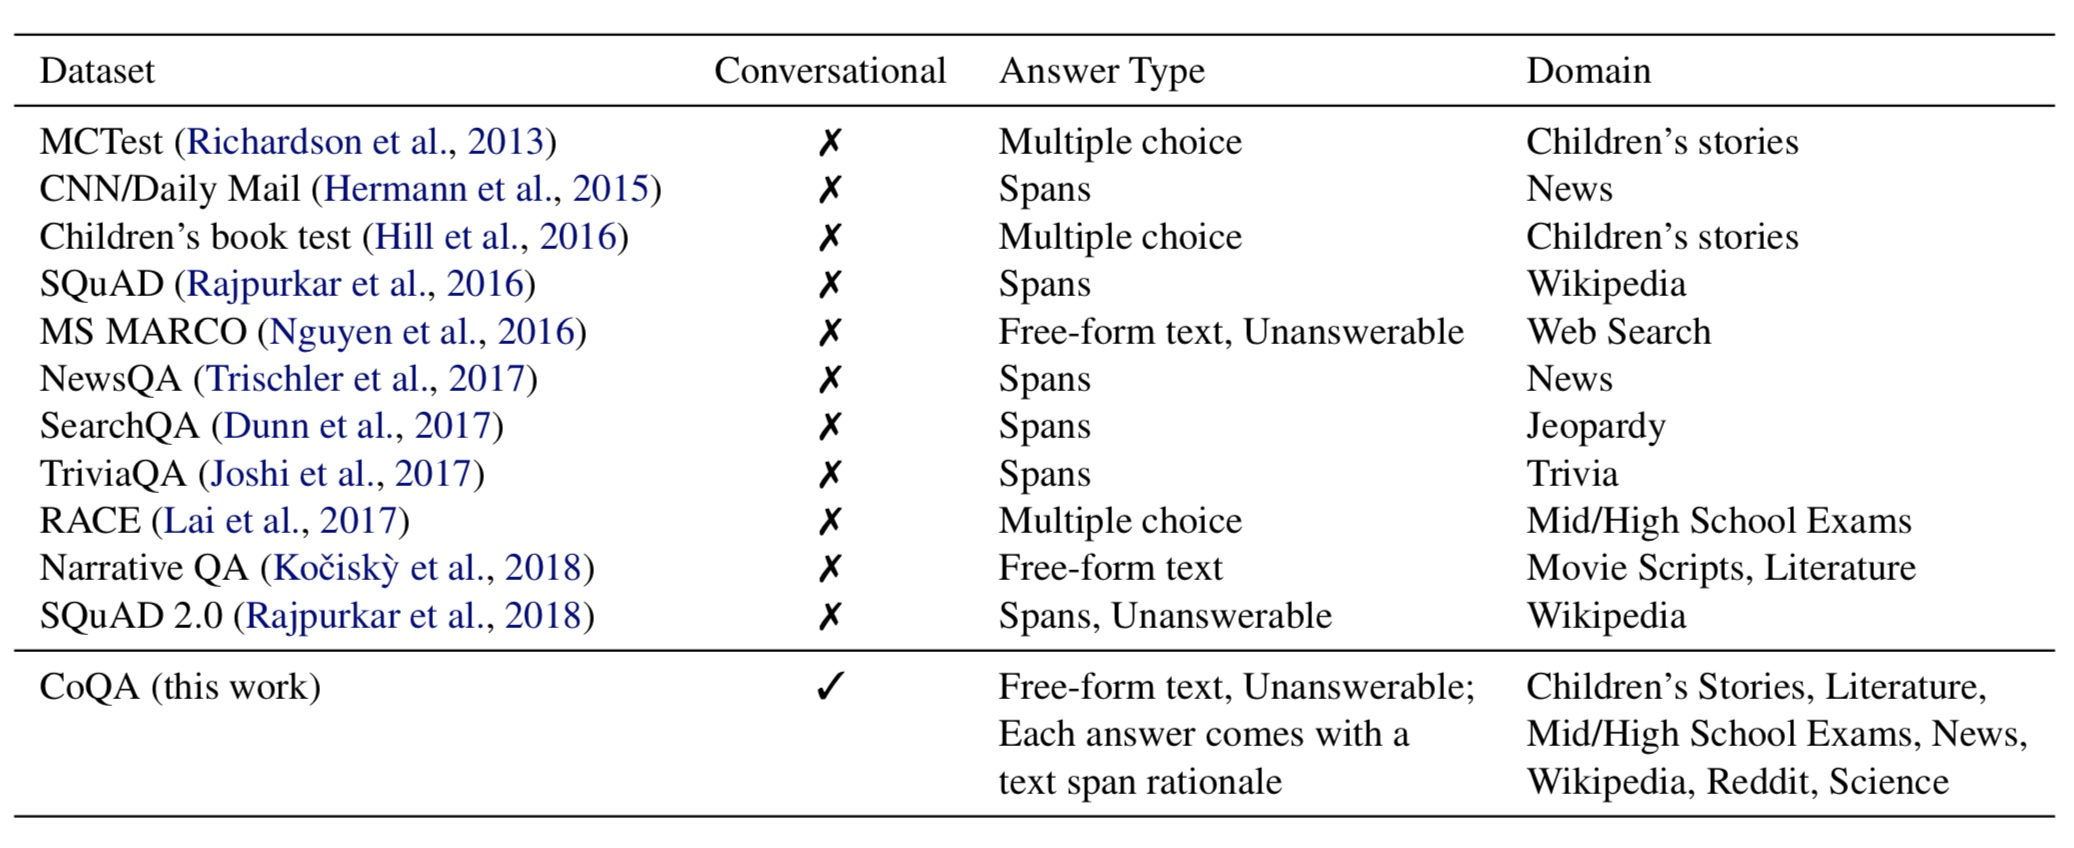
\includegraphics[width=0.9\textwidth]{table.jpeg}
    \caption{A Comparing between Existing Corpora and our Dataset.}
    \label{fig:TABLE}
\end{figure}


-- 











\chapter{Statistical Analysis}

Currently, I have collected 71 conversations, which contains 426 questions together with their answers, from 12 participants. The average length for the questions and answers is 6.8 and 5.1 separately. The word token ratio for the question is 0.2 which is less than 0.3 for answers. And the top 5 question words are what, when, and, who, where.

After I collect this dataset in the next three weeks, I will investigate how different contexts (e.g. there is a topic shift, the domain is unfamiliar) influences the appearance of different linguistics patterns within the dialogues.

\chapter{Modelling Coherent Dialogues Using Neural Networks}
I will write my proposed neural model here.

\chapter{Towards Building Coherent Open-domain Dialogue Systems}
I will investigate how to integrate the neural with an existing dialogue system. 

\chapter{Discussion}
I will discuss interesting findings from the above analysis and try to interpret them based on linguistic knowledge. 

\chapter{Conclusion and Future Work}

% use the following and \cite{} as above if you use BibTeX
% otherwise generate bibtem entries
\bibliographystyle{plain}
\bibliography{mybibfile}

\end{document}